\begin{auf}
    214
\end{auf}
Ein Vollzylinder vom Radius $R$ (Trägheitsmoment bezüglich der Zylinderachse $J_S =\frac{mR^2}{2}$) rollt aus der Ruhelage eine Strecke $s=2.5m$ auf der schiefen Ebene (Neigungswinkel $\alpha=20^\circ$) hinab.
\begin{enumerate}
    \item[\ref{eq:214_a}] Welche Geschwindigkeit hat der Zylinder unten?
    \item[\ref{eq:214_b}] Wie groß ist seine Beschleunigung und welche Zeit benötigt er für diese Strecke?
    \item[\ref{eq:214_c}] Welche Zeit benötigt im Vergleich dazu ein Hohlzylinder gleicher Masse, dessen Innenradius $r=\frac{9}{10}R$ beträgt? ($R$ Außenradius, Trägheitsmoment bezüglich der Zylinderachse $J_S=\frac{m(R^2 + r^2 )}{2}$.)
\end{enumerate}
\begin{figure}[h]
    \centering
    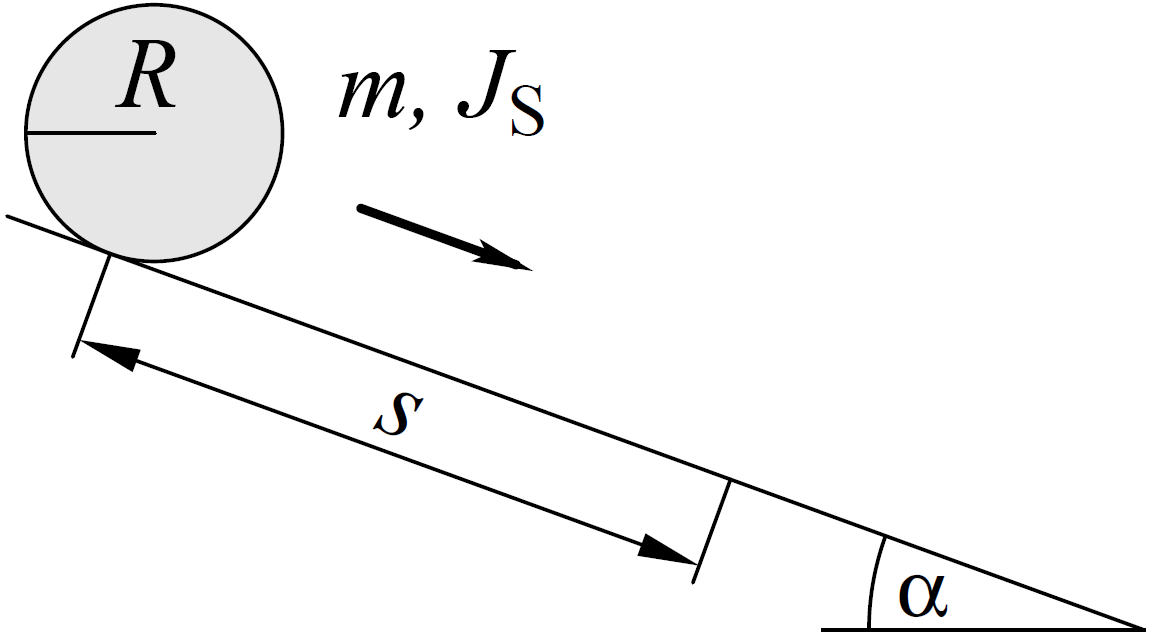
\includegraphics[width=0.7\linewidth]{images/214_0.png}
    \caption{Versuchsaufbau Aufgabe 214}
\end{figure}
Während des Herabrollen des Zylinders wird potentielle Energie $E_{Pot}$ in kinetische Energie $E_{Kin}$ und Rotationsenergie $E_{Rot}$ umgewandelt.
\begin{align*}
    E_{Pot}&=E_{kin}+E_{Rot}\\
    m\cdot g\cdot h&=\frac{m\cdot v^2}{2}+\frac{J_S\cdot\omega^2}{2}
\end{align*}
Dabei ist die Höhe $h=s\cdot\sin\alpha$, $J_S=\frac{m\cdot R^2}{2}$ und $\omega=\frac{v}{R}$.
\begin{align}
    m\cdot g\cdot s\cdot\sin\alpha&=\frac{m\cdot v^2}{2}+\frac{m\cdot R^2\cdot v^2}{4\cdot R^2}		\nonumber\\
    g\cdot s\cdot\sin\alpha&=\frac{v^2}{2}+\frac{v^2}{4}																		\nonumber\\
    g\cdot s\cdot\sin\alpha&=\frac{3}{4}v^2																								\nonumber\\
    v^2&=\frac{4\cdot g\cdot s\cdot\sin\alpha}{3}																						\nonumber\\
    v&=\sqrt{\frac{4\cdot g\cdot s\cdot\sin\alpha}{3}}																				\label{eq:214_velocity}\\
    v&=\sqrt{\frac{4\cdot 9.81\frac{m}{s^2}\cdot 2.5m\cdot\sin(20^\circ)}{3}}										\nonumber\\
    &\boxed{v=3.34\frac{m}{s}}	\tag{a}	\label{eq:214_a}
\end{align}
Es handelt sich um eine gleichmäßig beschleunigte Bewegung. Demnach gelten die folgenden Gleichungen.
\begin{align}
    v^2&=2\cdot a\cdot s	\nonumber\\
    a&=\frac{v^2}{2\cdot s}	\label{eq:214_acceleration}\\
    s&=\frac{a}{2}t^2		\nonumber\\
    t^2&=\frac{2s}{a}		\nonumber\\
    t&=\sqrt{\frac{2s}{a}}	\label{eq:214_time}
\end{align}
Man setzt \eqref{eq:214_velocity} in \eqref{eq:214_acceleration} ein. Im Anschluss setzt man diese Gleichung in \eqref{eq:214_time} ein.
\begin{align*}
    a&=\frac{\left(\sqrt{\frac{4\cdot g\cdot s\cdot\sin\alpha}{3}}\right)^2}{2\cdot s}\\
    a&=\frac{4\cdot g\cdot s\cdot\sin\alpha}{6\cdot s}\\
    a&=\frac{2\cdot g\cdot\sin\alpha}{3}\\
    t&=\sqrt{\frac{2s}{\frac{2\cdot g\cdot\sin\alpha}{3}}}\\
    t&=\sqrt{\frac{3s}{g\cdot\sin\alpha}}\\
    a&=\frac{2\cdot 9.81\frac{m}{s^2}\cdot\sin(20^\circ)}{3}\\
    t&=\sqrt{\frac{3\cdot2.5m}{9.81\frac{m}{s^2}\cdot\sin(20^\circ)}}\\
    &\boxed{a=2.24\frac{m}{s^2},\,t=1.50s}	\tag{b}	\label{eq:214_b}
\end{align*}
Für den Hohlzylinder bleibt die Ansatz der gleiche. Lediglich das Trägheitsmoment ändert sich.
\begin{align*}
    J_S&=\frac{m(R^2+r^2)}{2}\\
    r&=\frac{9}{10}R\\
    J_S&=\frac{m(R^2+\frac{81}{100}R^2)}{2}\\
    J_S&=\frac{181\cdot m\cdot R^2}{200}\\
    m\cdot g\cdot s\cdot\sin\alpha&=\frac{m\cdot v^2}{2}+\frac{181\cdot m\cdot R^2\cdot v^2}{400\cdot R^2}\\
    g\cdot s\cdot\sin\alpha&=\frac{v^2}{2}+\frac{181}{400}v^2\\
    g\cdot s\cdot\sin\alpha&=\frac{381}{400}v^2\\
    v&=\sqrt{\frac{400\cdot g\cdot s\cdot\sin\alpha}{381}}\\
    a&=\frac{\left(\sqrt{\frac{400\cdot g\cdot s\cdot\sin\alpha}{381}}\right)^2}{2\cdot s}\\
    a&=\frac{400\cdot g\cdot s\cdot\sin\alpha}{762\cdot s}\\
    a&=\frac{200\cdot g\cdot\sin\alpha}{381}\\
    t&=\sqrt{\frac{2s}{\frac{200\cdot g\cdot\sin\alpha}{381}}}\\
    t&=\sqrt{\frac{381s}{100\cdot g\cdot\sin\alpha}}\\
    t&=\sqrt{\frac{381\cdot2.5m}{100\cdot9.81\frac{m}{s^2}\cdot\sin(20^\circ)}}\\
    &\boxed{t=1.68s}	\tag{c}	\label{eq:214_c}
\end{align*}